% !TEX root = mainthesis.texx
%Appendix 
\appendix
\renewcommand{\thechapter}{C}
\renewcommand{\chaptername}{Appendix}

\chapter{Full derivation of the Raman coupled $\xyz$ states}
\label{app:Rashba_derivation}

In this Appendix I derive the full time-dependent Hamiltonian describing the Raman coupled $\xyz$ states. The system is based on the theoretical proposal~\cite implementation  If a rotating wave approximation is performed on the system we can derive Equation~\ref{Eq:Rashba_atoms}. \cite{}

We consider an $F=1$ system that is subject to a constant magnetic field $B_0\ez$ and an RF magnetic field $B_{RF}\cos(\omrf t)\ex$. The system is described by the Hamiltonian
\begin{equation}
\hat H_{RF} = \omega_0 \fz - \frac{\epsilon}{\hbar} (\fz^2-\mathbb{I})+2\Omrf\cos(\omrf t)\fx,
\label{Eq:H_RF}
\end{equation}
%
where $\omega_0 = g_F\mu_B B_0$ is the Larmor frequency, $\epsilon$ is a quadratic Zeeman shift that breaks the degeneracy of the $\ket{m_F=-1}\leftrightarrow$ $\ket{m_F=0}$ and $\ket{m_F=1}\leftrightarrow$ $\ket{m_F=0}$ transitions, and $\Omrf = g_F\mu_B B_{RF} / 2$ is the RF coupling strength. We then transform the Hamiltonian into a rotating frame using the unitary transformation $\hat U(t) = \exp(-i \omrf t \fz)$. The spin-1 operators under this transformation are
\begin{align}
\begin{split}
\fx  & \rightarrow \cos(\omrf t)\fx -\sin(\omrf t)\fy \\
     & = e^{i\omega_{RF}t}\fp +e^{-i\omega_{RF}t}\fm\\
\fy & \rightarrow \sin(\omrf t)\fx + \cos(\omrf t)\fy \\
     &=\frac{1}{i}(e^{i\omega_{RF}t}\fp-e^{-i\omega_{RF}t}\fm) \\
\fz & \rightarrow \fz.
\label{eq:rotation_transformations}
\end{split}
\end{align}
%
The unitary evolution in the rotating frame is described by the transformed Hamiltonian $\hat U^{\dagger}(t)(\hat H_{RF} -i \hbar \partial_t)\hat U(t)$, which after neglecting terms that are oscillating at $2\omrf$ is 

\begin{equation}
\hat H_{RWA}= \Delta \fz - \frac{\epsilon}{\hbar} (\fz^2-\mathbb{I}) + \Omrf \fx
\label{Eq:H_RWA}
\end{equation}
%

For $\Delta=0$, the eigenstates of Eq.~\ref{Eq:H_RWA} are 
\begin{align}
\begin{split}
\ket{x}=&-\frac{1}{\sqrt{2}}\ket{1}+\frac{1}{\sqrt{2}}\ket{-1}, \\
%
\ket{y} =& \frac{\Omega }{\sqrt{4 \Omega ^2-\epsilon  \sqrt{4 \Omega ^2+\epsilon ^2}+\epsilon ^2}}\ket{1}
,\frac{\sqrt{4 \Omega ^2+\epsilon ^2}-\epsilon }{\Omega 
   \sqrt{\frac{\left(\epsilon -\sqrt{4 \Omega ^2+\epsilon ^2}\right)^2}{\Omega ^2}+4}},\frac{\Omega }{\sqrt{4 \Omega ^2-\epsilon  \sqrt{4 \Omega
   ^2+\epsilon ^2}+\epsilon ^2}}, \\
%
\ket{z} =& \frac{\Omega }{\sqrt{-\Omega_* \epsilon +\Omega_*^2}}\ket{1} +\frac{\Omega_*-\epsilon }{\Omega  \sqrt{\frac{(\epsilon
   -\Omega_*)^2}{\Omega ^2}+4}}\ket{0} +\frac{\Omega }{\sqrt{-\Omega_* \epsilon +\Omega_*^2}}\ket{-1}.
\end{split}
\end{align}
\textcolor{red}{This can be probably written in a prettier form. Write in terms of big XYZ basis?}
%
The $\xyz$ states are linear combinations of $m_F$ states and therefore transitions between these states are not subjected to angular momentum selection rules. I will show later that all states can be coupled using a combination of the $\fx$, $\fy$, and $\fz$ operators in the lab frame. 

\subsection{Raman dressing of the RF eigenstates}

Our main goal is to engineer a Hamiltonian with Rashba SOC. It was shown in [Dan's PRA ref] that this can be done with a minimum of three states with nonzero Raman coupling matrix elements. The $\xyz$ RF dressed-states are therefore good candidates to construct the desired Rashba Hamiltonian as was shown in [Dan's Rashba RF paper].
%
In this section I will go through a lengthy  derivation of the Rashba Hamiltonian, without sweeping undesired off-resonant couplings under the rug.  For simplicity I will start this description in the lab frame and I will not make any initial assumptions about direction of propagation or frequency each of the beams. Consider three linearly polarized Raman beams propagating along the $xy$ plane as shown in Fig.~\ref{fig:Rashba_layout}. 
\begin{figure*}[hb]
	\begin{center}
		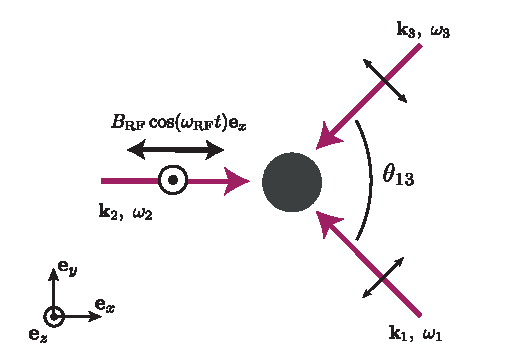
\includegraphics{Figures/AppendixC/Rashba_layout.pdf}
		\caption
		{Laser layout:  We use a strong RF field and three linearly polarized Raman beams propagating in the $xy$ plane couple the $\xyz$ states and engineer the Rashba Hamiltonian. 
		\label{fig:Rashba_layout}}
	\end{center}
\end{figure*}
%
The electric field at the atoms is
\begin{equation}
\mathbf{E}(x, t)=\sum_{i=1}^{3}E_i\mathbf{e}_i e^{i(\mathbf{k}_i\cdot\mathbf{x}-\omega_i t)},
\label{eq:Raman_basic}
\end{equation}
%
where $E_i$ is the field amplitude, $\omega_i$ is the angular frequency, and $\mathbf{e}_i$ is the polarization of each of the beams. In order to generate the necessary Raman couplings proportional to $\fx$, $\fy$ and $\fz$ we need two horizontally polarized Raman beams and one vertically polarized beam. Without loss of generality we choose
\begin{align}
\begin{split}
\mathbf{e}_1&=\frac{(k_{1y}, -k_{1x}, 0)}{\vert\vert \mathbf k_1 \vert\vert^2}, \\
\mathbf{e}_2&=(0, 0, 1), \\
\mathbf{e}_3&=\frac{(k_{3y}, -k_{3x}, 0)}{\vert\vert \mathbf k_3 \vert\vert^2}, \\
\label{eq:polarization}
\end{split}
\end{align}
%
The Raman Hamiltonian is given by the vector component of the Stark shift generated by the atom-light interaction
%
\begin{equation}
\hat{H}_R=(iu_v\mathbf E\times\mathbf E^*)\cdot\hat F,
\label{eq:vector_stark}
\end{equation}
%
where $u_v$ is the vector polarizability. Now let's expand Eq.~\ref{eq:vector_stark} using the field at the atoms from Eq.~\ref{eq:Raman_basic}.

\begin{align}
\begin{split}
\mathbf E\times\mathbf E^* &= (E_1^* \e_1 e^{-i(\mathbf k_1\cdot \mathbf x -\omega_1 t)}
					       +E_2^* \e_2 e^{-i(\mathbf k_2\cdot \mathbf x -\omega_2 t)} 
					       +E_3^* \e_3 e^{-i(\mathbf k_3\cdot \mathbf x -\omega_3 t)})
					       \times c.c \\
					  & = E_1^*E_2(\e_1\times \e_2)e^{i[(\k_2-\k_1)\cdot\x-(\omega_2-\omega_1)t]}
					      + E_1^*E_3(\e_1\times \e_3)e^{i[(\k_3-\k_1)\cdot\x-(\omega_3-\omega_1)t]} \\
					  & + E_2^*E_1(\e_2\times \e_1)e^{i[(\k_1-\k_2)\cdot\x-(\omega_1-\omega_2)t]}	 
					     + E_2^*E_3(\e_2\times \e_3)e^{i[(\k_3-\k_2)\cdot\x-(\omega_3-\omega_2)t]} \\
					  & + E_3^*E_1(\e_3\times \e_1)e^{i[(\k_1-\k_3)\cdot\x-(\omega_1-\omega_3)t]}
					     +  E_3^*E_2(\e_3\times \e_2)e^{i[(\k_2-\k_3)\cdot\x-(\omega_2-\omega_3)t]} \\
					  &=2i\big[ (\e_1\times\e_2) \text{Im}
					  	\{E_1^*E_2\ e^{i(\k_{21}\cdot \x - \omega_{21} t)}\} \\
					& +(\e_1\times\e_3) \text{Im}\{E_1^*E_3\ e^{i(\k_{32}\cdot \x - \omega_{32} t)}\} \\
					& +(\e_2\times\e_3) \text{Im}\{E_2^*E_3\ e^{i(\k_{32}\cdot \x - \omega_{32} t)}\} \big]
\end{split}
\end{align}
%
also from the definitions of the polarization vectors we can calculate the cross products
\begin{align}
\begin{split}
\e_1\times \e_2 &= \frac{(-k_{1x}, -k_{1y}, 0)}{\vert\vert \k_1\vert\vert^2} = -\hat\k_1 \\
\e_1\times \e_3 &= \frac{(0, 0, -k_{1y}k_{3x}+k_{3y}k_{1x})}{\vert\vert \k_1\vert\vert^2\vert\vert \k_3\vert\vert^2} = \ez\sin\theta_{13}\\
\e_2\times\e_3 &= \frac{(k_{3x}, k_{3y}, 0)}{\vert\vert \k_3\vert\vert^2} = \hat\k_3,
\end{split}
\end{align}
%
and putting everything together
\begin{align}
\begin{split}
iu_v\mathbf E^* \times\mathbf E \cdot\mathbf{\hat{F}}&= -2u_v\big[-\hat\k_1\text{Im}\{12\}+\ez\sin\theta_{13}\text{Im}\{13\}+\hat\k_3\text{Im}\{23\}\big] \cdot \hat{\mathbf{F}}\\
&=(\Omega_x, \Omega_y, \Omega_z)\cdot \hat{\mathbf{F}}
\label{eq:full_Raman}
\end{split}
\end{align}
%
with
\begin{align}
\begin{split}
\Omega_x &=\frac{k_{1x}}{\vert\vert\k_1\vert\vert}\text{Im}\{\Omega_{12}e^{i(\k_{21}\cdot\x-\omega_{21}t)}\}
		+\frac{k_{3x}}{\vert\vert\k_3\vert\vert}\text{Im}\{\Omega_{23}e^{i(\k_{32}\cdot\x-\omega_{32}t)}\}\\
\Omega_y &=\frac{k_{1y}}{\vert\vert\k_1\vert\vert}\text{Im}\{\Omega_{12}e^{i(\k_{21}\cdot\x-\omega_{21}t)}\}
		+\frac{k_{3y}}{\vert\vert\k_3\vert\vert}\text{Im}\{\Omega_{23}e^{i(\k_{32}\cdot\x-\omega_{32}t)}\}\\
\Omega_z &=\text{Im} \{\Omega_{13}e^{i(\k_{31}\cdot\x-\omega_{31}t)}\},
\end{split}
\end{align} 
and
\begin{align}
\begin{split}
\Omega_{12}&=2u_vE_1^*E_2 \\
\Omega_{13}&=-2u_vE_1^*E_3\sin\theta_{13}\\
\Omega_{23}&=-2u_vE_2^*E_3.
\end{split}
\end{align}

\subsubsection{Going into rotating frame}

This is where things start getting fun. We need to transform Eq.~\ref{eq:full_Raman} into the rotating frame. Which terms are `slow' and we get to keep and which are `fast' depends on the specific choice of Raman frequencies. Only the $\fx$ and $\fy$ operators are affected by the unitary transformation while $\fz$ remains unchanged. We therefore choose the beams that give a $\fz$ coupling to be close in frequency. 



\begin{figure*}[hb]
	\begin{center}
		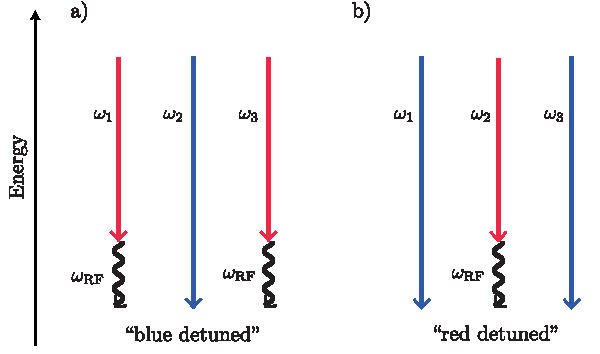
\includegraphics{Figures/AppendixC/laser_frequencies.pdf}
		\caption
		{Laser frequencies:  We have two frequency choices that allow us to address the three transitions between the $\xyz$ states. {\bf{a)}} The blue detuned case. There are 2 frequencies smaller by about $\omega_{RF}$ and one larger frequency. {\bf{b)}} The red detuned case. There are 2 frequencies that are larger by about $\omega_{RF}$ and one smaller frequency. Nice!
		\label{fig:Rashba_frequencies}}
	\end{center}
\end{figure*}
%
There are two different frequency choices which Dan calls `blue' and `red' detuned which are shown in Fig.~\ref{fig:Rashba_frequencies}, and they determine wether $\omega_{21}$ and $\omega_{31}$ are positive or negative. 
%
I'm not sure if we can generalize something at this point. Lets look at the firs term of the $\Omega_x\fx$ coupling for practice. 
\begin{align}
\begin{split}
\Omega_x ^{(1)}\fx &\rightarrow\frac{1}{4i}\frac{k_{1x}}{\vert\vert\k_1\vert\vert}
\left(\Omega_{12}e^{i(\k_{21}\cdot\x-\omega_{21})t} - \Omega_{12}^*e^{-i(\k_{21}\cdot\x-\omega_{21}t)}\right)\left(e^{i\omega_{RF}t}\fp +e^{-i\omega_{RF}t}\fm\right) \\
& \approx \frac{1}{4i}\frac{k_{1x}}{\vert\vert\k_1\vert\vert}
\left(\Omega_{12}e^{i(\k_{21}\cdot\x-(\omega_{21}\mp\omega_{RF})t)}\hat{F}_{\pm} 
- \Omega_{12}^*e^{-i(\k_{21}\cdot\x-(\omega_{21}\mp \omega_{RF})t)}\hat{F}_{\mp}\right) \\
& = \frac{1}{4i}\frac{k_{1x}}{\vert\vert\k_1\vert\vert}
\left(\Omega_{12}e^{i(\k_{21}\cdot\x-(\omega_{21}\mp\omega_{RF})t)}-c.c.\right)\fx
\pm i\left(\Omega_{12}e^{i(\k_{21}\cdot\x-(\omega_{21}\mp\omega_{RF})t)}+c.c.\right)\fy \\
& = \frac{1}{2}\frac{k_{1x}}{\vert\vert\k_1\vert\vert}\vert\Omega_{12}\vert
\left(\sin[\k_{21}\cdot\x-(\omega_{21}\mp\omega_{RF})t+\phi_{12}]\fx\pm\cos[\k_{21}\cdot\x-(\omega_{21}\mp\omega_{RF})t+\phi_{12}]\fy\right)
\end{split}
\end{align} 
Where the upper sign corresponds to the $\omega_{21}>0$ case (blue detuned) and the lower sign to $\omega_{21}<0$ (red detuned). Similarly, the second therm of $\Omega_x\fx$ is
\begin{align}
\begin{split}
\Omega_x ^{(2)}\fx &\rightarrow\frac{1}{4i}\frac{k_{3x}}{\vert\vert\k_3\vert\vert}
\left(\Omega_{23}e^{i(\k_{32}\cdot\x-\omega_{32})t} - \Omega_{23}^*e^{-i(\k_{32}\cdot\x-\omega_{32}t)}\right)\left(e^{i\omega_{RF}t}\fp +e^{-i\omega_{RF}t}\fm\right) \\
& \approx  \frac{1}{2}\frac{k_{3x}}{\vert\vert\k_3\vert\vert}\vert\Omega_{23}\vert
\left(\sin[\k_{32}\cdot\x-(\omega_{32}\mp\omega_{RF})t+\phi_{23}]\fx\pm\cos[\k_{32}\cdot\x-(\omega_{32}\mp\omega_{RF})t+\phi_{23}]\fy\right)
\end{split}
\end{align}
%
where I used the same sign convention as before. It is important to keep in mind though that if $\omega_{21}$ is positive then $\omega_{32}$ must be negative and vice versa. \textcolor{red}{Double check again that signs are correct!}
%
Let's continue with the algebra galore...
\begin{align}
\begin{split}
\Omega_y^{(1)}\fy& \rightarrow -\frac{1}{4}\frac{k_{1y}}{\vert\vert\k_1\vert\vert}
\left(\Omega_{12}e^{i(\k_{21}\cdot\x-\omega_{21}t} - \Omega_{12}^*e^{-i(\k_{21}\cdot\x-\omega_{21}t)}\right)
\left(e^{i\omega_{RF}t}\fp-e^{-i\omega_{RF}t}\fm\right) \\
& = \mp\frac{1}{4}\frac{k_{1y}}{\vert\vert\k_1\vert\vert} 
\left(\Omega_{12}e^{i(\k_{21}\cdot\x-(\omega_{21}\mp\omega_{RF})t)}\hat{F}_{\pm} 
+ \Omega_{12}^*e^{-i(\k_{21}\cdot\x-(\omega_{21}\mp \omega_{RF})t)}\hat{F}_{\mp}\right) \\
&=\mp\frac{1}{4}\frac{k_{1y}}{\vert\vert\k_1\vert\vert} 
\left(\left(\Omega_{12}e^{i(\k_{21}\cdot\x-(\omega_{21}\mp\omega_{RF})t)} + c.c.\right)\fx 
+ i\left(\Omega_{12}e^{i(\k_{21}\cdot\x-(\omega_{21}\mp\omega_{RF})t)} - c.c.\right)\fy \right) \\
&= \mp\frac{1}{2}\frac{k_{1y}}{\vert\vert\k_1\vert\vert} 
\vert\Omega_{12}\vert\left(\cos[\k_{21}\cdot\x-(\omega_{21}\mp\omega_{RF})t+\phi_{12}]\fx
-\sin[\k_{21}\cdot\x-(\omega_{21}\mp\omega_{RF})t+\phi_{12}]\fy\right),
\end{split}
\end{align}
%
and
\begin{align}
\begin{split}
\Omega_y^{(2)}\fy& \rightarrow -\frac{1}{4}\frac{k_{3y}}{\vert\vert\k_3\vert\vert}
\left(\Omega_{23}e^{i(\k_{32}\cdot\x-\omega_{32}t} - \Omega_{23}^*e^{-i(\k_{32}\cdot\x-\omega_{32}t)}\right)
\left(e^{i\omega_{RF}t}\fp-e^{-i\omega_{RF}t}\fm\right) \\
&\approx \mp\frac{1}{2}\frac{k_{3y}}{\vert\vert\k_3\vert\vert} 
\vert\Omega_{23}\vert\left(\cos[\k_{32}\cdot\x-(\omega_{32}\mp\omega_{RF})t+\phi_{23}]\fx
-\sin[\k_{32}\cdot\x-(\omega_{32}\mp\omega_{RF})t+\phi_{23}]\fy\right).
\end{split}
\end{align}
%
The complete Hamiltonian in the rotating frame after doing the rotating wave approximation is then
%
\begin{align}
\begin{split}
\hat{H}= \frac{1}{2}\frac{\vert\Omega_{12}\vert}{\vert\vert\k_1\vert\vert}
\Bigg(&\Big(k_{1x}\sin[\k_{21}\cdot\x-(\omega_{21}\mp\omega_{RF})t+\phi_{12}]
\pm k_{1y}\cos[\k_{21}\cdot\x-(\omega_{21}\pm\omega_{RF})t+\phi_{12}]\Big)\fx \\
+ &\Big(\pm k_{1x}\cos[\k_{21}\cdot\x-(\omega_{21}\mp\omega_{RF})t+\phi_{12}]
\mp k_{1y}\sin[\k_{21}\cdot\x-(\omega_{21}\pm\omega_{RF})t+\phi_{12}]\Big)\fy\Bigg) \\
\frac{1}{2}\frac{\vert\Omega_{23}\vert}{\vert\vert\k_3\vert\vert}
\Bigg(&\Big(k_{3x}\sin[\k_{32}\cdot\x-(\omega_{32}\mp\omega_{RF})t+\phi_{23}]
\pm k_{3y}\cos[\k_{32}\cdot\x-(\omega_{32}\pm\omega_{RF})t+\phi_{23}]\Big)\fx \\
+ &\Big(\pm k_{3x}\cos[\k_{32}\cdot\x-(\omega_{32}\mp\omega_{RF})t+\phi_{23}]
\mp k_{3y}\sin[\k_{32}\cdot\x-(\omega_{32}\pm\omega_{RF})t+\phi_{23}]\Big)\fy \Bigg)\\
+&\vert\Omega_{13}\vert\sin(\k_{31}\cdot\x - \omega_{31}t+\phi_{13})\fz
\end{split}
\end{align}
%

\begin{figure*}[htb]
\begin{center}
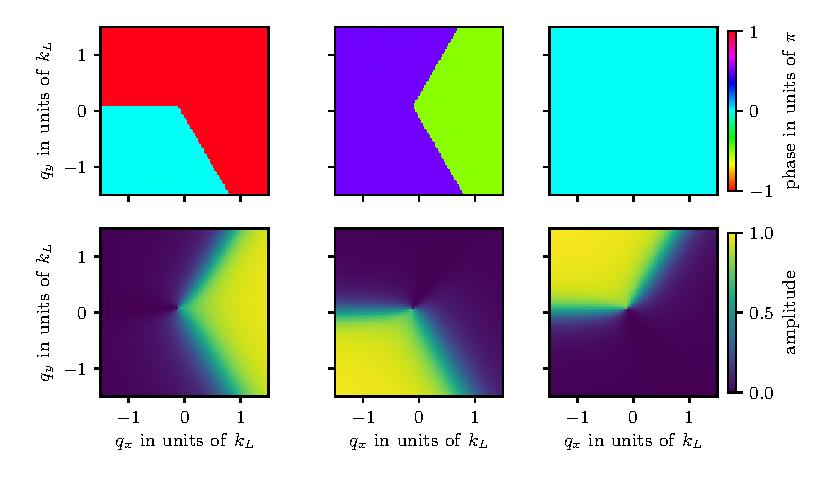
\includegraphics[]{Figures/Chapter8/topological_eigenvecs.pdf}
\caption{{\bfseries a} Probabilities as a function of quasimomentum for the three output ports of the interferometer at $t_{\rm free}=\unit[160]{\mu s}$ {\bfseries b} Probabilities as a function of free evolution time $t_{\mathrm{free}}$ for an input state with quasimomentum $(q_1, q_2)=(0.55,-0.92)\,k_{\rm L}$ indicated by the blue star on {\bfseries a} and in the topological ground branch ($n=1$)}
\label{fig:topological_eigenvecs}
\end{center}
\end{figure*}

\begin{figure*}[htb]
\begin{center}
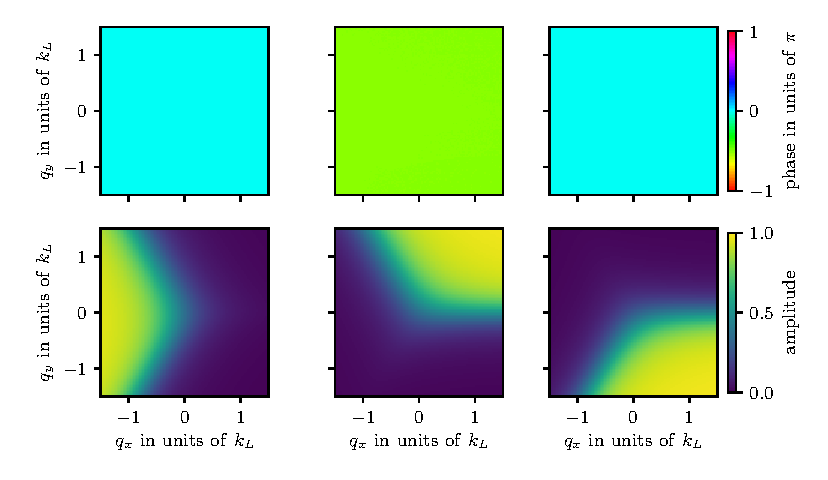
\includegraphics[]{Figures/Chapter8/nontopological_eigenvecs.pdf}
\caption{{\bfseries a} Probabilities as a function of quasimomentum for the three output ports of the interferometer at $t_{\rm free}=\unit[160]{\mu s}$ {\bfseries b} Probabilities as a function of free evolution time $t_{\mathrm{free}}$ for an input state with quasimomentum $(q_1, q_2)=(0.55,-0.92)\,k_{\rm L}$ indicated by the blue star on {\bfseries a} and in the topological ground branch ($n=1$)}
\label{fig:nontopological_eigenvecs}
\end{center}
\end{figure*}
